\begin{equation}
    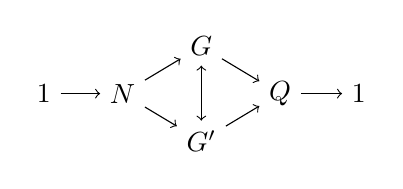
\begin{tikzpicture}
        \node (A) at (-2,0) {$1$};
        \node (B) at (-1,0) {$N$};
        \draw[->] (A) -- (B);
        \node (C) at (0, 0.6) {$G$};
        \node (D) at (0, -0.6) {$G'$};
        \draw [<->] (C) -- (D);
        \draw [->] (B) -- (C);
        \draw [->] (B) -- (D);
        \node (E) at (1, 0) {$Q$};
        \draw [->] (C) -- (E);
        \draw [->] (D) -- (E);
        \node (F) at (2, 0) {$1$};
        \draw [->] (E) -- (F);
    \end{tikzpicture}
\end{equation}